\documentclass[border=3pt]{standalone}
% Preâmbulo compartilhado pelos diagramas TikZ da aula 11 (Localização por Grade e Monte Carlo)
\usepackage[T1]{fontenc}
\usepackage[utf8]{inputenc}
\usepackage{lmodern}
\usepackage{amsmath}
\usepackage{xcolor}
\usepackage{tikz}
\usetikzlibrary{arrows.meta,angles,quotes,decorations.pathmorphing,calc,
                positioning,shapes.geometric,shapes.misc,backgrounds,fit,
                math}

% Paleta (mesma dos SVGs originais)
\definecolor{dblue}{HTML}{2A5B8C}
\definecolor{dorange}{HTML}{B3541E}
\definecolor{dgreen}{HTML}{4A7C59}
\definecolor{dred}{HTML}{9C4B4B}
\definecolor{dcream}{HTML}{F4F1EA}
\definecolor{dshade}{HTML}{DDD7C9}

% Função gaussiana (não normalizada por padrão de escala visual)
\pgfmathdeclarefunction{gauss}{3}{%
  \pgfmathparse{1/(#3*sqrt(2*pi))*exp(-((#1-#2)^2)/(2*#3^2))}%
}

% Estilos comuns (prefixo d... para não colidir com chaves internas do pgf)
\tikzset{
  >={Stealth[length=2mm]},
  dguide/.style={gray!55, dashed, line width=0.4pt},
  daxis/.style={gray!60, line width=0.7pt, ->},
  dbody/.style={fill=black!3, draw=black!80, line width=1pt},
  dacc/.style={draw=dblue, line width=1pt},
  dlbl/.style={black!55, font=\small},
  dsub/.style={black!45, font=\footnotesize},
  dstate/.style={circle, draw=black!80, fill=dcream, line width=1pt,
                 minimum size=17mm, font=\large, inner sep=1pt},
  dobs/.style={circle, draw=black!80, fill=dshade, line width=1pt,
               minimum size=14mm, font=\large, inner sep=1pt},
  dbox/.style={rounded corners=2pt, draw=black!80, fill=dcream, line width=1pt,
               align=center, inner sep=6pt},
  dop/.style={circle, draw=black!80, fill=white, line width=1pt,
              minimum size=6mm, inner sep=0pt, font=\small},
  dtrans/.style={->, dblue, line width=1pt},
  dmeas/.style={->, dorange, line width=1pt},
  dcurve/.style={line width=1pt, dblue},
  dcurveb/.style={line width=1.4pt, dorange},
}

\begin{document}
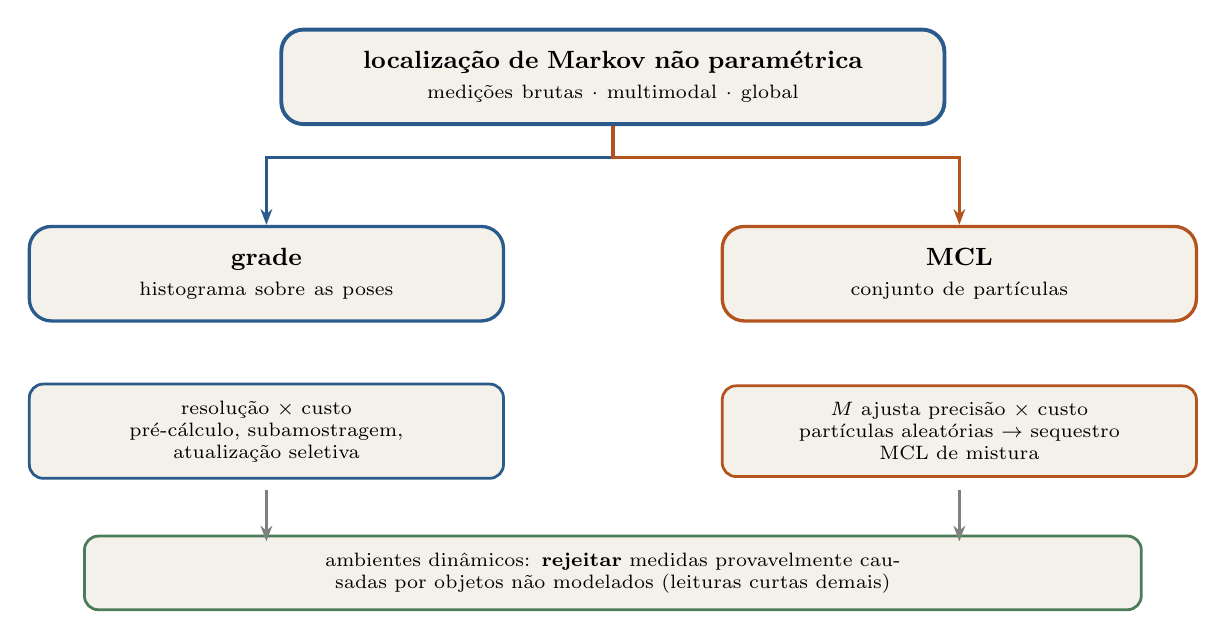
\begin{tikzpicture}[x=1cm,y=1cm,
   n/.style={dbox, rounded corners=8pt, text width=5.6cm, minimum height=1.2cm, font=\small}]
  \node[n, draw=dblue, line width=1.4pt, text width=8cm] (r) at (6.2,5.4) {\textbf{localização de Markov não paramétrica}\\ \scriptsize medições brutas $\cdot$ multimodal $\cdot$ global};
  \node[n, draw=dblue, line width=1.2pt] (g) at (1.8,2.9) {\textbf{grade}\\ \scriptsize histograma sobre as poses};
  \node[n, draw=dorange, line width=1.2pt] (m) at (10.6,2.9) {\textbf{MCL}\\ \scriptsize conjunto de partículas};
  \draw[dtrans, line width=1.2pt] (r.south) -- ++(0,-0.4) -| (g.north); \draw[dmeas, line width=1.2pt] (r.south) -- ++(0,-0.4) -| (m.north);
  \node[dbox, rounded corners=5pt, text width=5.6cm, font=\scriptsize, draw=dblue] at (1.8,0.9) {resolução $\times$ custo\\ pré-cálculo, subamostragem,\\ atualização seletiva};
  \node[dbox, rounded corners=5pt, text width=5.6cm, font=\scriptsize, draw=dorange] at (10.6,0.9) {$M$ ajusta precisão $\times$ custo\\ partículas aleatórias $\to$ sequestro\\ MCL de mistura};
  \node[dbox, rounded corners=5pt, text width=13cm, font=\scriptsize, draw=dgreen] at (6.2,-0.9) {ambientes dinâmicos: \textbf{rejeitar} medidas provavelmente causadas por objetos não modelados (leituras curtas demais)};
  \draw[->, black!50, line width=0.9pt] (1.8,0.15) -- (1.8,-0.5); \draw[->, black!50, line width=0.9pt] (10.6,0.15) -- (10.6,-0.5);
\end{tikzpicture}
\end{document}
